\section{tooltip()}\label{specimen-tooltip}

Short local explanation positioned near the thing it describes, for cases where the meaning is helpful but not part of the document flow.

\begin{center}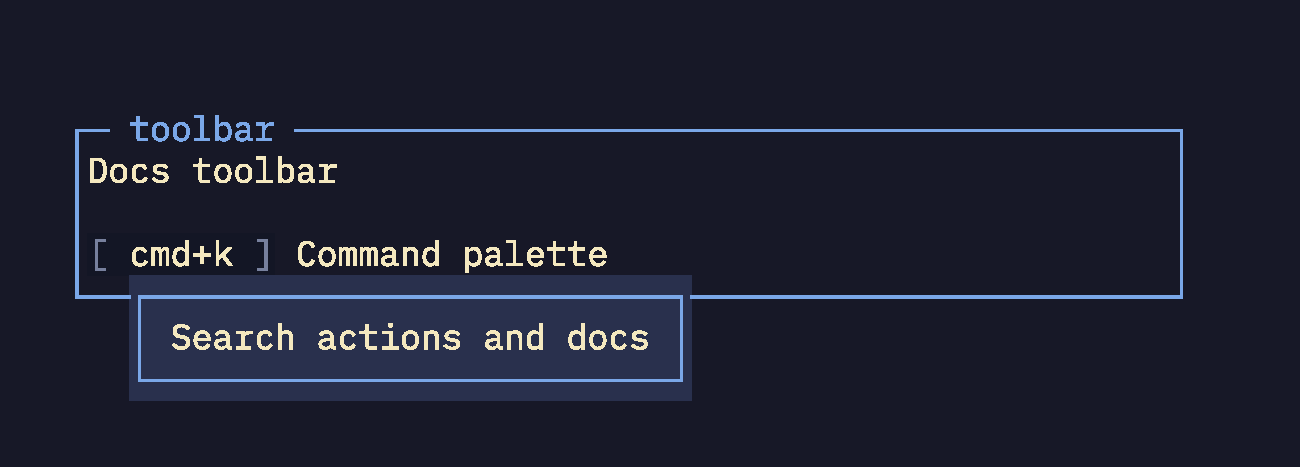
\includegraphics[width=\linewidth,height=.62\textheight,keepaspectratio]{figures/tooltip.pdf}\end{center}

{\footnotesize\color{BookMuted}Story: \path{tooltip}; variant: \path{local-explanation}; 60 × 10 cells.\par}\medskip

